% This is part of the Jabuti 1.0 Manual.
% Copyright 2003 (c) Auri Marcelo Rizzo Vicenzi, Marcio Eduardo Delamaro,
% Jose Carlos Maldonado.
% See the file FDL.TXT for copying conditions.

\section{\toolname Functionality and Graphical
Interface}\label{sec:tool}

\toolname implements a subset of the functionalities provided by
\xSuds, a complete tool suite for C and C++
programs~\cite{Agrawal98MSTA}. This section describes the
operations that can be performed by \toolname. The graphical
interface allows the beginner to explore and learn the concepts of
control-flow and data-flow testing. Moreover, it provides a better
way to visualize which part of the classes under testing are
already covered and which are not. A general view of the \toolname
graphical interface, including its menus, is presented in
Figure~\ref{fig:tool}. A brief description of each option on each
menu is presented below.

% This is part of the Jabuti 1.0 Manual.
% Copyright 2003 (c) Auri Marcelo Rizzo Vicenzi, Marcio Eduardo Delamaro,
% Jose Carlos Maldonado.
% See the file FDL.TXT for copying conditions.

\begin{figure}[!ht]
\begin{center}
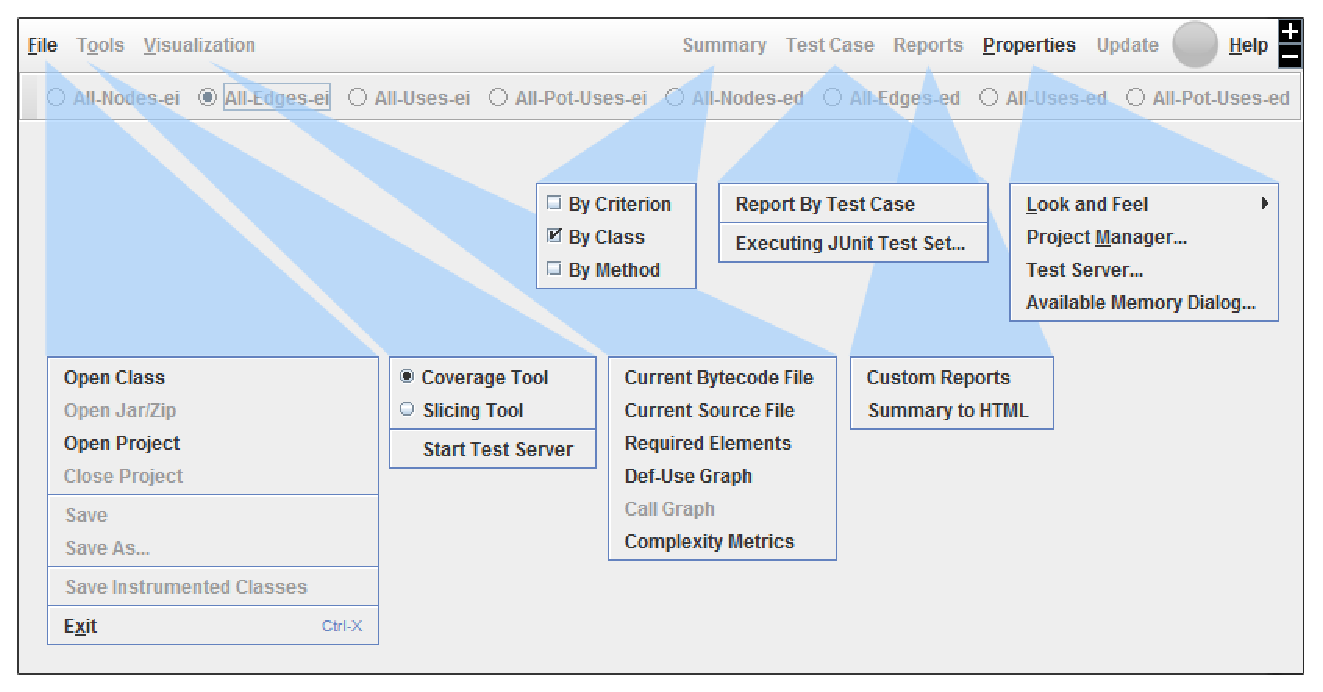
\includegraphics[width=0.7\textwidth]{fig/main-window-editted.eps}
\caption{\label{fig:tool}Operations available in the graphical
interface.}
\end{center}
\end{figure}


\begin{itemize}
    \item \textbf{File Menu} - provides options to create and
    manipulate a \toolname project.
        \begin{itemize}
            \item \textbf{Open Class} - allows to select the base class
            file from where the classes to be tested are
            identified.

            \item \textbf{Open Project} - opens a previously created
            project.

            \item \textbf{Close Project} - closes the current
            project.

            \item \textbf{Save} - saves the current project.

            \item \textbf{Save As} - saves the current project with a different
            name.
            
            \item \textbf{Save Instrumented Classes} - saves the classes from 
            current project, already instrumented for external testing.

            \item \textbf{Exit} - exits of the tool.
        \end{itemize}

    \item \textbf{Tools} - provides the set of tools available in
    \toolname.
        \begin{itemize}
            \item \textbf{Coverage Tool} - enables the \toolname coverage
            tool.

            \item \textbf{Slicing Tool} - enables the \toolname slicing
            tool.
            
            \item \textbf{Start Test Server} - starts the test server for
            mobile devices.

        \end{itemize}

    \item \textbf{Visualization} - provides different forms of
    visualization of the classes and methods under testing.
        \begin{itemize}
            \item \textbf{Current Bytecode File} - shows the highlighted bytecode of the
            current selected class file.

            \item \textbf{Current Source File} - shows the highlighted source code of the
            current selected class file. Observe that this option requires that the source
            code is available to be performed.

            \item \textbf{Required Elements} - shows the set of required elements
            for a given method of a given class, considering the current selected
            criterion (shown below the main menu). The presented
            screen also allows to mark a testing requirement as active/deactive or
            feasible/infeasible.

            \item \textbf{Def-Use Graph} - shows the \DUG
            of a given method of the current class.

            \item \textbf{Complexity Metrics} - shows the resultant value of
            the set of complexity metrics implemented in \toolname for the
            complete set of user classes obtained from the base class.
            This set of classes includes the classes under testing.
        \end{itemize}

    \item \textbf{Summary} - provides personalized coverage information
        in different levels of abstractions.
        \begin{itemize}
            \item \textbf{By Criterion} - shows the cumulative coverage
            information for each testing criterion, considering all classes
            under testing.

            \item \textbf{By Class} - shows the coverage
            information with respect to the current selected criterion,
            for each individual class under testing.

            \item \textbf{By Method} - shows the coverage
            information with respect to the current selected criterion,
            for each individual method of each class under testing.
        \end{itemize}

    \item \textbf{Test Case} - provides options for test set
    manipulation and report generation.
        \begin{itemize}
            \item \textbf{Report By Test Case} - shows the coverage
            information with respect to the current selected criterion,
            for each individual test case, considering all class under
            testing. The presented screen also allows to enable/disable and
            delete/undelete test cases.

%            \item \textbf{Report By Test Case Path} - shows the coverage
%            information with respect to the current selected criterion,
%            for each individual test case path, considering all class under
%            testing.

            \item \textbf{Importing from JUnit} - allows to import a test set
            generated according to the JUnit framework.
        \end{itemize}

    \item \textbf{Reports} - provides options to save \toolname's reports in
    HTML format.
        \begin{itemize}
            \item \textbf{Custom Reports} - allows to generate a custom
            HTML report from the current testing project considering different
            levels of granularity.

            \item \textbf{Summary to HTML} - allows to generate a HTML from
            any tabled style report provided by the \toolname graphical interface.
        \end{itemize}

    \item \textbf{Properties} - provides general configuration options.
        \begin{itemize}
            \item \textbf{Look and Feel} - allows to change the
            look and feel style considering three different options:
            Metal (default), Motif, and Windows.

            \item \textbf{Project Manager...} - allows to verify and change
            the current set of classes under testing in the current project.
            
            \item \textbf{Test Server...} - configuration of the test server.
            
            \item \textbf{Available Memory Dialog...} - shows current available
            memory on system.
        \end{itemize}

    \item \textbf{Update} - provides a visual information every time an
    event that affect the coverage occurs. For example, such a button becomes
    red in case additional test cases are imported or appended in the end of the
    trace file to indicate that a new event that affects the coverage information
    occurs. As soon as it is clicked, its background color changes
    to grey.

    \item \textbf{Help} - provides only one option to show information
    about the authors/developers of \toolname.
\end{itemize}

\toolname requires the creation of a testing project, such that
the tester can specify only once the set of classes to be
instrumented and tested. Section~\ref{sec:project} describes how
to create a \toolname's testing project. After having created the
project, \toolname provides to the tester a coverage analysis
tool, a slicing tool and a static metric measure tool. The
coverage analysis tool is described in Section~\ref{sec:coverage}.
Section~\ref{sec:slice} describes the slicing tool, and
Section~\ref{sec:metrics} describes the measure tool.
